% SPHEREx Blink, release documentation
% NASA Space Apps Challenge 2026, Milano, team Observationally Speaking
% Build: tectonic spherex-blink.tex
\documentclass[11pt,a4paper]{article}

\usepackage[T1]{fontenc}
\usepackage[utf8]{inputenc}
\usepackage{lmodern}
\usepackage[margin=2.4cm]{geometry}
\usepackage{amsmath,amssymb}
\usepackage{siunitx}
\usepackage{booktabs,tabularx}
\usepackage{enumitem}
\usepackage{xcolor}
\usepackage{listings}
\usepackage{tikz}
\usetikzlibrary{arrows.meta,positioning}
\usepackage[hidelinks]{hyperref}

% ---------------------------------------------------------------- release facts
% Fill these in before tagging the release.
\newcommand{\Version}{v1.0.0}
\newcommand{\ReleaseDate}{15 November 2026}
\newcommand{\TeamName}{Observationally Speaking}
\newcommand{\Members}{Jessica Syafaq Muthmaina \\ Joowon Sohn}
\newcommand{\Repo}{\url{https://github.com/yourastrophysicist/SPHEREx-site}}
\newcommand{\ProjectPage}{\url{https://www.yourastro.space/SPHEREx/}}

\definecolor{siteblue}{HTML}{141EF0}
\sisetup{detect-all}
\lstset{basicstyle=\ttfamily\small, columns=fullflexible, frame=single,
        framerule=0.3pt, rulecolor=\color{gray}, breaklines=true}
\setlist{itemsep=2pt, topsep=4pt}

\hypersetup{pdftitle={SPHEREx Blink \Version},
            pdfauthor={\TeamName, NASA Space Apps Milano 2026}}

\begin{document}

% ---------------------------------------------------------------- title page
\begin{titlepage}
  \centering
  \vspace*{2cm}
  {\large NASA Space Apps Challenge 2026 \par}
  {\large Local event: Milano, Politecnico di Milano, 14 and 15 November 2026 \par}
  \vspace{2.2cm}
  {\Huge\bfseries\color{siteblue} SPHEREx Blink \par}
  \vspace{0.5cm}
  {\Large A blink viewer for the public SPHEREx images \par}
  \vspace{0.4cm}
  {\large Release \Version, technical documentation \par}
  \vspace{2.2cm}
  {\large Team \textbf{\TeamName} \par}
  \vspace{0.4cm}
  {\Members \par}
  \vfill
  \begin{tabular}{rl}
    Release date & \ReleaseDate \\
    Source code  & \Repo \\
    Project page & \ProjectPage \\
  \end{tabular}
  \vspace{1cm}
\end{titlepage}

\begin{abstract}
\noindent
SPHEREx Blink is a public web tool that shows the same small patch of sky in every
SPHEREx visit, one after the other, like a flipbook. The user gives a position on the sky,
and optionally a proper motion. The tool asks the NASA/IPAC Infrared Science Archive (IRSA)
which SPHEREx exposures cover that position, downloads small cutouts, subtracts the
zodiacal light, flags bad pixels and resamples every exposure onto one fixed north-up grid.
On that grid the field stars stand still, so anything that moves or changes brightness
stands out to the eye. The design follows WiseView, the blink tool of Backyard Worlds:
Planet 9. Every setting lives in the page URL, so one link is one view and can be shared.
This document describes release \Version: what the tool does, how the data path works,
how to run it, how it was tested on the five targets named by the challenge, and what it
cannot do.
\end{abstract}

\tableofcontents
\newpage

% =================================================================
\section{The challenge and our answer}

The challenge asked for a public-facing web tool. The user enters a right ascension and a
declination, and the tool plays the SPHEREx images of that patch as a short video, so that
moving objects are easy to spot. It named five test targets: Barnard's Star, Epsilon Indi B,
WISE 0855$-$0714, RW Aurigae and R Draconis. It pointed to WiseView as a model.

SPHEREx (Spectro-Photometer for the History of the Universe, Epoch of Reionization and Ices
Explorer) was launched on 12 March 2025. It maps the whole sky every six months with six
detectors between \SI{0.75}{\micro\metre} and \SI{5.0}{\micro\metre}. Each detector sits
behind a linear variable filter, so the wavelength changes across the array, and one star
seen in two exposures is in general seen at two slightly different wavelengths. The
pixels are large, about \ang{;;6.15}. This makes SPHEREx a good survey for slow, bright,
infrared movers such as nearby stars and brown dwarfs, and a hard one for faint fast
objects.

Our answer has three parts.
\begin{enumerate}
  \item A \textbf{data path} in Python, one function call from coordinates to a list of
        aligned frames (Section~\ref{sec:data}).
  \item A small \textbf{server} that wraps that call in one JSON endpoint and serves the page
        (Section~\ref{sec:server}).
  \item A \textbf{web page} that blinks the frames with WiseView-style controls and keeps every
        setting in the URL (Section~\ref{sec:page}).
\end{enumerate}

\begin{figure}[h]
\centering
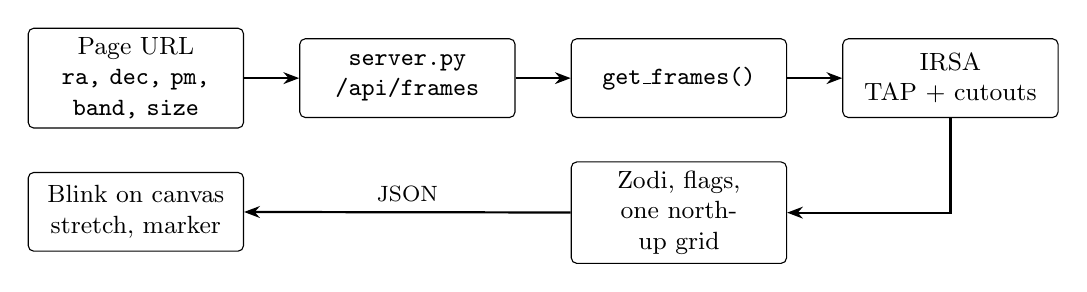
\begin{tikzpicture}[node distance=0.55cm and 0.7cm,
    box/.style={draw, rounded corners=2pt, align=center, font=\small,
                minimum height=1.0cm, text width=2.5cm},
    arr/.style={-{Stealth[length=2mm]}, thick}]
  \node[box] (url) {Page URL\\ \texttt{ra, dec, pm,}\\ \texttt{band, size}};
  \node[box, right=of url] (api) {\texttt{server.py}\\ \texttt{/api/frames}};
  \node[box, right=of api] (gf) {\texttt{get\_frames()}};
  \node[box, right=of gf] (irsa) {IRSA\\ TAP + cutouts};
  \node[box, below=of gf] (grid) {Zodi, flags,\\ one north-up grid};
  \node[box, below=of url] (blink) {Blink on canvas\\ stretch, marker};
  \draw[arr] (url) -- (api);
  \draw[arr] (api) -- (gf);
  \draw[arr] (gf) -- (irsa);
  \draw[arr] (irsa) |- (grid);
  \draw[arr] (grid) -- node[above, font=\footnotesize] {JSON} (blink);
\end{tikzpicture}
\caption{The path from a link to the blink.}
\end{figure}

% =================================================================
\section{The data path}\label{sec:data}

All of this is in \texttt{tool/spherex\_frames.py}. The public entry point is
\begin{lstlisting}[language=Python]
frames, grid = get_frames(ra, dec, band="D1", fov=0.03, epoch=2016.0,
                          pmra=0.0, pmdec=0.0, name="target", mask=True)
\end{lstlisting}
It returns the common grid as an \texttt{astropy} WCS and a list of frames, oldest first.
Each frame holds the image on the grid, the variance, the date (MJD and decimal year),
the wavelength at the target, the index of the six-month pass it belongs to, the predicted
pixel of the target at that date, and the archive URI of the exposure.

\subsection{Which exposures}
The archive is queried through IRSA's TAP service with ADQL. A row is kept when the
footprint polygon of the exposure contains the target and the detector matches:
\begin{lstlisting}[language=SQL]
SELECT a.uri, p.time_bounds_lower
FROM spherex.artifact a JOIN spherex.plane p ON a.planeid = p.planeid
WHERE 1 = CONTAINS(POINT('ICRS', ra, dec), p.poly)
  AND p.energy_bandpassname = 'SPHEREx-D1'
ORDER BY p.time_bounds_lower
\end{lstlisting}
The position used in the query is the target's position at 2026.0. The answer is cached on
disk for 24 hours, because the query alone takes about 20 seconds and new SPHEREx data reach
the archive about once a week.

\subsection{Moving the target to each date}
Positions from Gaia DR3 are given at epoch J2016.0. A star with a large proper motion is
many SPHEREx pixels away from that position by the time SPHEREx looks at it, so the
position is moved to the date of each exposure. Over a few years a linear motion is enough:
\begin{equation}
  \alpha(t) = \alpha_0 + \frac{\mu_{\alpha*}\,(t - t_0)}{\cos\delta_0},
  \qquad
  \delta(t) = \delta_0 + \mu_\delta\,(t - t_0),
\end{equation}
with $(\alpha_0,\delta_0)$ at epoch $t_0$, $\mu_{\alpha*} = \mu_\alpha\cos\delta$ and
$\mu_\delta$ in \si{mas.yr^{-1}}, converted to degrees. Parallax is not applied. For
Barnard's Star the parallax is \SI{0.55}{\arcsecond}, about a tenth of a pixel, and it shows
up as a small wobble on top of the straight walk.

\subsection{Cutouts}
For each exposure a cutout centred on the moved position is asked from IRSA's image
service. The cutout side is the field of view plus the distance the target travels over
the whole time span plus two pixels:
\begin{equation}
  s = \mathrm{fov} + \Delta t \, \sqrt{\mu_{\alpha*}^2 + \mu_\delta^2} + 2\,p,
  \qquad p = \ang{;;6.15},
\end{equation}
so that the fixed grid is covered at every date even though the cutout centre moves.
Downloads run in four parallel threads. The archive sometimes answers with a 503 or sends a
file cut short, so each download is checked for the five extensions the tool needs
(\texttt{IMAGE}, \texttt{FLAGS}, \texttt{VARIANCE}, \texttt{ZODI}, \texttt{WCS-WAVE}) and
retried with an exponential back-off up to eight times. One exposure that still fails is
skipped and logged instead of stopping the whole view.

\subsection{Cleaning each exposure}
\begin{itemize}
  \item \textbf{Zodiacal light.} The \texttt{ZODI} extension, the pipeline's model of the
        zodiacal light, is subtracted from \texttt{IMAGE}. Without this the sky level changes
        from visit to visit and the blink flickers.
  \item \textbf{Bad pixels.} A pixel is flagged when any of the flag bits 0, 1, 6, 9, 10,
        11, 15, 17 or 19 is set, the same set used in our prep script
        \texttt{coadd\_spherex.py}. With \texttt{mask=True} flagged pixels become NaN. The
        viewer asks with \texttt{mask=0} by default, because the saturated core of a bright
        star is flagged and a blink is easier to read when the star is still drawn.
  \item \textbf{Wavelength at the target.} The spectral WCS (\texttt{WCS-WAVE}, key
        \texttt{W}) gives the wavelength at the target's pixel, reported with every frame.
\end{itemize}

\subsection{One grid for every frame}
The grid is a gnomonic (TAN) projection, north up and east left, with SPHEREx-sized pixels.
It is centred on the target's position at the mean date of all exposures and has an odd
number of pixels per side, $N = \mathrm{round}(\mathrm{fov}/p)$ rounded up to odd, so that
the centre falls on a pixel. Because the grid is fixed on the sky and not on the target, the
field stars stay still and a moving target walks across the grid. For every grid pixel the
sky position is converted to the pixel coordinates of the exposure through the exposure's
own WCS, and the image is sampled there with bilinear interpolation. The variance is
sampled with nearest neighbour, so it is not smoothed.

\subsection{Passes}
SPHEREx covers a given point in visits a few days long, about six months apart. The frames
are split into passes wherever two consecutive exposures are more than 60 days apart. The
pass index is what the viewer uses for its default mode (Section~\ref{sec:page}).

% =================================================================
\section{The server}\label{sec:server}

\texttt{tool/server.py} uses the Python standard library only, besides the packages the
data path already needs (\texttt{numpy}, \texttt{scipy}, \texttt{astropy}). It serves the
page in \texttt{tool/web/} and one endpoint:
\begin{lstlisting}
GET /api/frames?ra=..&dec=..&size=..&band=..&epoch=..&pmra=..&pmdec=..&name=..&mask=..
\end{lstlisting}
Inputs are checked ($0 \le \alpha < 360$, $-90 \le \delta \le 90$, field side between 20
and 600 arcsec, detector D1 to D6) and a bad input returns HTTP 400 with the reason. An
archive failure returns HTTP 502 with the error text, so the page can tell the user what
went wrong. Results are kept in memory per view, and when the same view is asked twice at
once the second request waits for the first download instead of starting its own.

% =================================================================
\section{The page}\label{sec:page}

The page (\texttt{tool/web/index.html} and \texttt{app.js}) draws the frames on a canvas,
pixel for pixel, with no smoothing.

\paragraph{Two modes.} In \texttt{pass} mode, the default, each pass is reduced to its
per-pixel median, and the blink steps through the passes. This removes most cosmic rays
and single-exposure artefacts, and it matches the six-month rhythm in which a proper motion
becomes visible. In \texttt{frames} mode every exposure is shown on its own, with its date,
pass, wavelength and file name.

\paragraph{Stretch.} Each image is stretched on its own, so the change of brightness with
wavelength between exposures does not swamp the blink. The sky level $m$ is the median of
the finite pixels and the noise is the scaled median absolute deviation,
$\sigma = 1.4826\,\mathrm{MAD}$. In the default \texttt{asinh} stretch a pixel value $v$
becomes
\begin{equation}
  t = \frac{\operatorname{arsinh}\big((v - \ell)/\beta\big)}
           {\operatorname{arsinh}\big((h - \ell)/\beta\big)},
  \qquad \ell = m - 2\sigma, \quad \beta = 3\sigma,
\end{equation}
clipped to $[0,1]$, where $h$ is the upper percentile set by the \texttt{contrast}
parameter. This keeps faint field stars visible next to a saturated bright one. A linear
stretch between two percentiles is also available.

\paragraph{Marker and compass.} A red marker of four short ticks, with a gap in the middle so
it never covers the object, shows where the target should be at each date. N and E labels
show the orientation.

\paragraph{The URL is the state.} As in WiseView, every setting is a URL parameter, and the
URL is rewritten when a control changes. Table~\ref{tab:params} lists them. Presets fill in
the position, motion and detector for the five challenge targets, for example
\texttt{/?target=Barnard}.

\begin{table}[h]
\centering
\small
\begin{tabularx}{\linewidth}{@{}l X l@{}}
\toprule
Parameter & Meaning & Default \\
\midrule
\texttt{target} & preset name: \texttt{Barnard}, \texttt{EpsIndB}, \texttt{WISE0855}, \texttt{RWAur}, \texttt{RDra} & \\
\texttt{ra}, \texttt{dec} & position in degrees at \texttt{epoch} & \\
\texttt{pmra}, \texttt{pmdec} & proper motion in \si{mas.yr^{-1}} & 0 \\
\texttt{epoch} & epoch of the position, decimal year & 2016.0 \\
\texttt{size} & field side in arcsec & 108 \\
\texttt{band} & SPHEREx detector, D1 to D6 & D1 \\
\texttt{mode} & \texttt{pass} (median of each pass) or \texttt{frames} (every exposure) & \texttt{pass} \\
\texttt{speed} & blink interval in ms & 500 \\
\texttt{stretch} & \texttt{asinh} or \texttt{linear} & \texttt{asinh} \\
\texttt{contrast} & upper percentile of the stretch & 99.5 \\
\texttt{invert}, \texttt{marker}, \texttt{mask} & 1 or 0 & 0, 1, 0 \\
\bottomrule
\end{tabularx}
\caption{URL parameters. Keyboard: space plays or pauses, the arrow keys step.}
\label{tab:params}
\end{table}

% =================================================================
\section{Running it}

\begin{lstlisting}[language=bash]
git clone https://github.com/yourastrophysicist/SPHEREx-site
cd SPHEREx-site/tool
conda activate astrolab2      # any Python 3.10+ with numpy, scipy, astropy
python server.py
# open http://localhost:8000/?target=Barnard
\end{lstlisting}
The first view of a new field asks IRSA for every exposure and downloads the cutouts. This
takes a few minutes, and up to ten when the archive is busy. The files are then kept in
\texttt{\textasciitilde/spherex\_data} (or the folder in \texttt{\$SPHEREX\_DATA}) and the
same view opens in seconds. The port can be changed with \texttt{\$PORT}.

% =================================================================
\section{Tests on the challenge targets}

Table~\ref{tab:targets} gives the inputs of the five presets. Positions and motions are from
Gaia DR3 at J2016.0, except WISE 0855$-$0714, which is too faint for Gaia and uses the AllWISE
position with the motion of Kirkpatrick et al.\ (2021). The detector is the one where the
target is easiest to see.

\begin{table}[h]
\centering
\small
\begin{tabular}{@{}lrrrrrc@{}}
\toprule
Target & $\alpha$ (deg) & $\delta$ (deg) & epoch & $\mu_{\alpha*}$ & $\mu_\delta$ & detector \\
 & & & & \multicolumn{2}{c}{(\si{mas.yr^{-1}})} & \\
\midrule
Barnard's Star   & 269.448503 &   4.739420 & 2016.0  &  $-801.6$ & 10362.4 & D1 \\
Epsilon Indi B   & 331.076453 & $-56.793812$ & 2016.0  &  3982.0 & $-2466.8$ & D5 \\
WISE 0855$-$0714 & 133.794760 &  $-7.245146$ & 2010.56 & $-8123.7$ &  673.2 & D6 \\
RW Aurigae       &  76.956081 &  30.401205 & 2016.0  &     2.6 &  $-27.4$ & D1 \\
R Draconis       & 248.167378 &  66.755007 & 2016.0  &  $-20.6$ &    6.1 & D3 \\
\bottomrule
\end{tabular}
\caption{The five presets.}
\label{tab:targets}
\end{table}

\paragraph{Barnard's Star, D1.} 60 exposures over 3 passes, on a $19\times19$ grid
(\SI{108}{\arcsecond} field). The measured position of the star sits \SI{0.06}{px} from the
position predicted by the proper motion, which checks the alignment and the motion
correction together. The core of the star is saturated and flagged (57 grid pixels in the
masked view), which is why the viewer draws unmasked pixels by default. In the blink the
star walks north by about \SI{10.4}{\arcsecond} per year, which is \SI{0.85}{px} per
six-month pass, and the walk is plain to see over the three passes.

\paragraph{WISE 0855$-$0714, D6.} The coldest known brown dwarf is faint at SPHEREx's longest
wavelengths but visible in the pass medians. The preset opens a wider field,
\SI{216}{\arcsecond}, to give more field stars to judge against.

\paragraph{RW Aurigae and R Draconis.} These two barely move. They are in the set to show
the other half of the job: a young variable star and a Mira variable whose brightness
changes between passes while the field around them stays the same.

% =================================================================
\section{What it can and cannot find}

Published forecasts put a single SPHEREx exposure at roughly $V \approx 17$ for a point
source at 5$\sigma$ per channel, and the all-sky map after four passes at about AB 19.5 to
19.9 (deeper near the ecliptic poles). These are forecasts, not our measurements. The blink works on single passes, so its
practical limit is close to the single-exposure depth.

Behind the challenge sits the question of a distant ``Planet X''. For a planet seen in reflected
sunlight at opposition the flux falls as $r^{-4}$:
\begin{equation}
  m = m_\odot - 2.5 \log_{10} \frac{A_g R_p^2}{r^2 \Delta^2},
  \qquad m_\odot = -26.74\ (V),
\end{equation}
with the radius $R_p$ and the distances $r$ and $\Delta \approx r$ in AU and $A_g$ the
geometric albedo. A planet of three Earth radii with $A_g = 0.3$ is at $V \approx 18.8$ at
300 AU and $V \approx 21.0$ at 500 AU. That is fainter than a single SPHEREx exposure, so this
tool will not find a Planet Nine of the usual size and distance, and we say so on the page.
What it does well is the thing SPHEREx is suited for: nearby stars and brown dwarfs with
large proper motions, and variable stars, at infrared wavelengths and on the whole sky.

\paragraph{Known limits of \Version.}
\begin{itemize}
  \item Linear proper motion only, no parallax.
  \item One detector at a time. The wavelength changes slightly between exposures because of
        the linear variable filter. It is reported, not corrected.
  \item The first view of a new field is slow because the cutouts come from IRSA live.
  \item The server is meant to run locally or behind a single host. It has no rate limiting.
\end{itemize}

% =================================================================
\section{Use of earlier work and of AI}

\paragraph{Earlier work.} The data path grows out of two prep scripts and a notebook made by
Jessica Syafaq Muthmaina on 10 November 2026, before the event, to check that the SPHEREx
data could be reached. The TAP query, the proper-motion centring, the retrying download and
the flag mask come from there. The Milano Local Lead confirmed on 14 November 2026 that this
earlier work may be used. It is kept apart in the \texttt{prep/} folder of the repository,
with its own README and guide.

\paragraph{AI.} Parts of the code and of this document were written with help from Claude
(Anthropic). The team chose the method, checked the results against the archive and the
expected motions, and is responsible for the content.

% =================================================================
\section{Credits and data use}

\begin{itemize}
  \item \textbf{SPHEREx} Level 2 spectral images: NASA/JPL-Caltech/IPAC, through the NASA/IPAC
        Infrared Science Archive (IRSA).
  \item \textbf{Gaia} DR3: European Space Agency, mission Gaia, processed by the Gaia Data
        Processing and Analysis Consortium (DPAC).
  \item \textbf{AllWISE}: NASA/JPL-Caltech, UCLA. Motion of WISE 0855$-$0714 from Kirkpatrick
        et al.\ (2021).
  \item \textbf{WiseView} (Caselden et al.), used as the model for the interface.
  \item Software: NumPy, SciPy, Astropy.
\end{itemize}
NASA does not endorse this project. Data are used under the terms of each archive.

% =================================================================
\sloppy
\section*{References}
\addcontentsline{toc}{section}{References}
\begin{enumerate}[label={[\arabic*]}, leftmargin=*]
  \item Bock, J.\ et al., SPHEREx mission, NASA/JPL-Caltech/IPAC,
        \url{https://spherex.caltech.edu}.
  \item NASA/IPAC Infrared Science Archive, SPHEREx data and tutorials,
        \url{https://irsa.ipac.caltech.edu} and \url{https://caltech-ipac.github.io/irsa-tutorials}.
  \item Gaia Collaboration, Vallenari, A.\ et al.\ 2023, \textit{Gaia Data Release 3: Summary of
        the content and survey properties}, A\&A 674, A1.
  \item Kirkpatrick, J.\,D.\ et al.\ 2021, \textit{The field substellar mass function based on
        the full-sky 20 pc census of 525 L, T, and Y dwarfs}, ApJS 253, 7.
  \item Caselden, D.\ et al.\ 2018, \textit{WiseView: Visualizing motion and variability of
        faint WISE sources}, Astrophysics Source Code Library, ascl:1806.004.
  \item Astropy Collaboration 2022, \textit{The Astropy Project: Sustaining and growing a
        community-oriented open-source project and the latest major release (v5.0)},
        ApJ 935, 167.
  \item Earlier work: \texttt{prep/} in \Repo, 10 November 2026.
\end{enumerate}

\end{document}
